\pgfplotsset{every axis/.append style={tick label style={/pgf/number format/fixed},font=\scriptsize,ylabel near ticks,xlabel near ticks,grid=major}}

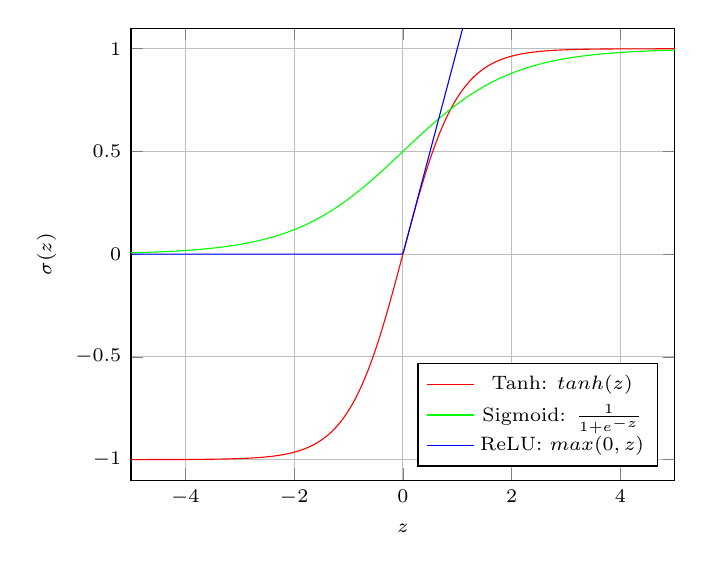
\begin{tikzpicture}
    \begin{axis}[width=0.7\textwidth,ylabel=$\sigma(z)$,xlabel=$z$,ymin=-1.1,ymax=1.1,xmin=-5,xmax=5,legend pos=south east, samples=300]
        \addplot[red,smooth] {tanh(x)};
        \addplot[green,smooth] {1/(1+exp(-x))};
        \addplot[blue,smooth] {max(0,x)};
        \addlegendentry{Tanh: $tanh(z)$}
        \addlegendentry{Sigmoid: $\frac{1}{1+e^{-z}}$}
        \addlegendentry{ReLU: $max(0, z)$}
    \end{axis}
\end{tikzpicture}